%
% This is the LaTeX template file for lecture notes for EE 382C/EE 361C.
%
% To familiarize yourself with this template, the body contains
% some examples of its use.  Look them over.  Then you can
% run LaTeX on this file.  After you have LaTeXed this file then
% you can look over the result either by printing it out with
% dvips or using xdvi.
%
% This template is based on the template for Prof. Sinclair's CS 270.

\documentclass[twoside]{article}
\usepackage{graphics}
\usepackage{graphicx}
\setlength{\oddsidemargin}{0.25 in}
\setlength{\evensidemargin}{-0.25 in}
\setlength{\topmargin}{-0.6 in}
\setlength{\textwidth}{6.5 in}
\setlength{\textheight}{8.5 in}
\setlength{\headsep}{0.75 in}
\setlength{\parindent}{0 in}
\setlength{\parskip}{0.1 in}

%
% The following commands set up the lecnum (lecture number)
% counter and make various numbering schemes work relative
% to the lecture number.
%
\newcounter{lecnum}
\renewcommand{\thepage}{\thelecnum-\arabic{page}}
\renewcommand{\thesection}{\thelecnum.\arabic{section}}
\renewcommand{\theequation}{\thelecnum.\arabic{equation}}
\renewcommand{\thefigure}{\thelecnum.\arabic{figure}}
\renewcommand{\thetable}{\thelecnum.\arabic{table}}

%
% The following macro is used to generate the header.
%
\newcommand{\lecture}[4]{
   \pagestyle{myheadings}
   \thispagestyle{plain}
   \newpage
   \setcounter{lecnum}{#1}
   \setcounter{page}{1}
   \noindent
   \begin{center}
   \framebox{
      \vbox{\vspace{2mm}
    \hbox to 6.28in { {\bf EE 382V: Parallel Algorithms
                        \hfill Fall 2017} }
       \vspace{4mm}
       \hbox to 6.28in { {\Large \hfill Lecture #1: #2  \hfill} }
       \vspace{2mm}
       \hbox to 6.28in { {\it Lecturer: #3 \hfill Scribe: #4} }
      \vspace{2mm}}
   }
   \end{center}
   \markboth{Lecture #1: #2}{Lecture #1: #2}
   %{\bf Disclaimer}: {\it These notes have not been subjected to the
   %usual scrutiny reserved for formal publications.  They may be distributed
   %outside this class only with the permission of the Instructor.}
   \vspace*{4mm}
}

%
% Convention for citations is authors' initials followed by the year.
% For example, to cite a paper by Leighton and Maggs you would type
% \cite{LM89}, and to cite a paper by Strassen you would type \cite{S69}.
% (To avoid bibliography problems, for now we redefine the \cite command.)
% Also commands that create a suitable format for the reference list.
\renewcommand{\cite}[1]{[#1]}
\def\beginrefs{\begin{list}%
        {[\arabic{equation}]}{\usecounter{equation}
         \setlength{\leftmargin}{2.0truecm}\setlength{\labelsep}{0.4truecm}%
         \setlength{\labelwidth}{1.6truecm}}}
\def\endrefs{\end{list}}
\def\bibentry#1{\item[\hbox{[#1]}]}

%Use this command for a figure; it puts a figure in wherever you want it.
%usage: \fig{NUMBER}{SPACE-IN-INCHES}{CAPTION}
\newcommand{\fig}[3]{
			\vspace{#2}
			\begin{center}
			Figure \thelecnum.#1:~#3
			\end{center}
	}
% Use these for theorems, lemmas, proofs, etc.
\newtheorem{theorem}{Theorem}[lecnum]
\newtheorem{lemma}[theorem]{Lemma}
\newtheorem{proposition}[theorem]{Proposition}
\newtheorem{claim}[theorem]{Claim}
\newtheorem{corollary}[theorem]{Corollary}
\newtheorem{definition}[theorem]{Definition}
\newenvironment{proof}{{\bf Proof:}}{\hfill\rule{2mm}{2mm}}

% **** IF YOU WANT TO DEFINE ADDITIONAL MACROS FOR YOURSELF, PUT THEM HERE:

\begin{document}
%FILL IN THE RIGHT INFO.
%\lecture{**LECTURE-NUMBER**}{**DATE**}{**LECTURER**}{**SCRIBE**}
\lecture{18}{November 4}{Vijay Garg}{My Luc}
%\footnotetext{These notes are partially based on those of Nigel Mansell.}

% **** YOUR NOTES GO HERE:

% Some general latex examples and examples making use of the
% macros follow.  
%**** IN GENERAL, BE BRIEF. LONG SCRIBE NOTES, NO MATTER HOW WELL WRITTEN,
%**** ARE NEVER READ BY ANYBODY.
\section{Introduction}
A compute system has two parts: program and data. For data, when a bit gets corrupted, it will behave badly. The question is if it will continue to behave badly or come back to normal/legal state.  A self-stabilizing system is guaranteed to come back to a normal/legal state after a finite number of moves.\\
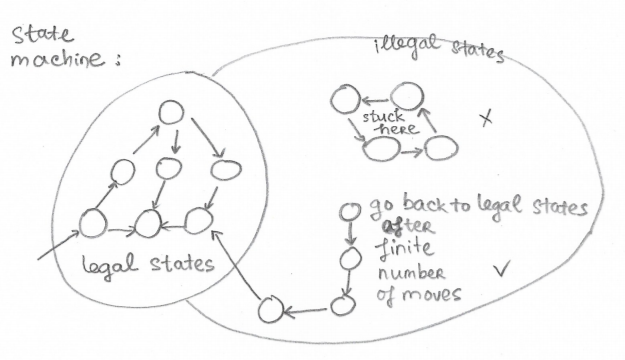
\includegraphics[scale=0.6]{statemachine.PNG}

\section{Mutual Exclusion with K-state Machines}

A machine can enter critical section only if it has privilege. The goal of the self-stabilizing mutual exclusion algorithm is to determine who has the privilege and how the privileges move in the network. Self-stabilizing algorithm ensures that sooner or later the system will be in a configuration in which only 1 process has the privilege to enter the critical section. \\
\\
Assume:\\
N: number of machines 0\ldots N-1. Each machine is a K-state machine. \\
S: state of the machine 0\ldots K-1 (K $\geq$ N) \\
K: number of labels using in the system (K $\geq$ N) \\
L: left neighbor \\\\\\\\\\\\\\\\\\\\\\
\textbf{Bottom machine: if (L = S) then S := S+1 mod K }
(The bottom machine has privilege if L = S. When it is done with the critical section, it updates S := S+1 mod K) \\
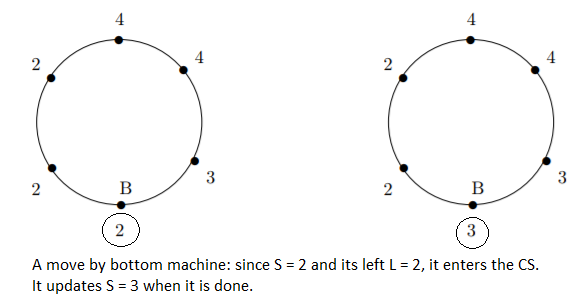
\includegraphics[scale=0.6]{bottom.PNG} \\

\textbf{Normal machine: if (L $\neq$ S) then S := L}
(Normal machine has privilege if L $\neq$ S. When it is done with the critical section, it updates S := L) \\\\
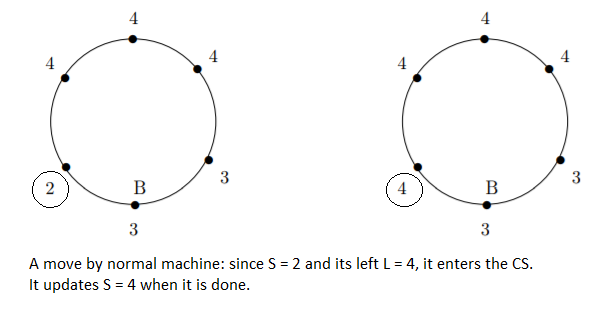
\includegraphics[scale=0.6]{normal.PNG} \\\\

There are 2 legal states:\\
1.	All states are the same: in this case the bottom machine has the privilege\\
2.	Some consecutive states are the same to a certain point m and then different from that point on: in this case the normal machine m+1 has the privilege.

\subsection{Claim 1}
\textbf{Any sequence of moves in which the bottom machine does not move is finite.}\\\\
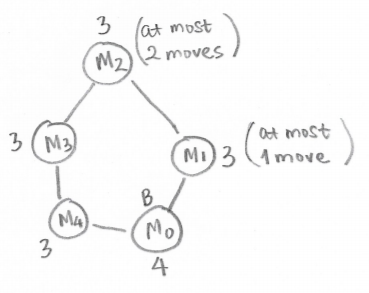
\includegraphics[scale=0.6]{claim1.PNG}\\
Normal machine i can move at most i times.\\
Total number of moves is finite: 1 + 2 + 3 + \ldots + N-1 = O(${N}^2$)\\


\subsection{Claim 2}

\textbf{In any configuration, either:\\
1.	Bottom machine has unique label or\\
2.	There is a label missing from the network.}\\\\
There are N machines, so at least N labels are used. If a label is not unique, then some other machine must have the same label. Therefore, some labels must be missing.\\

\subsection{Claim 3}

\textbf{Within finite number of move, "Bottom machine has unique label" must be true.}\\\\
If (L = S) then S := S+1 mod K. The bottom machine is cycling labels from 0, 1, 2, \ldots, K-1, 0, 1, 2,  \ldots, K-1, 0, 1, \ldots 
The bottom machine is the only machine that generates labels. Normal machines copy label from its left.\\
Within a finite number of moves, the bottom machine has to move, as soon as the bottom machine gets to the missing label, it has unique label.

\subsection{Theorem}
For all configurations, the system will get into a legal state in a finite number of moves.

\section{Application}

Routing table gets corrupted: a package is looping in a circle. Routing table needs to be designed in a way that eventually the package reaches its destination.




\end{document}





